\subsection{Merkmalsextraktion} \label{merkmalsextraftion-1}

Wie bereits in Kapitel \ref{merkmalsextraktion-0} beschrieben, ist das Ziel der Merkmalsextraktion Charakteristiken und Merkmale in den Daten zu finden, die für das
Klassifizierungsproblem von möglichst hoher Relevanz sind. Im Rahmen des ELISE Projektes haben wir verschiedene Vorgehensweisen angewendet. Im den folgenden Unterkapiteln werden diese vorgestellt. \\



% Unterkapitel 
\subsubsection{Handgefertigte Merkmale} \label{hc-features-1}
Der handgefertigten Merkmal Ansatz (enlg. "hand-crafted features approach") besteht in der Berechnung relativ einfacher Merkmale von denen vermudetet wird, dass sie für das Klassifizierungsproblem der Eingangssignale relevant sein können. Diese Vorgehensweise hat den Vorteil des einfachen Aufbaus als auch der relativ geringen benötigten Rechenleistung, wobei potentiell gute Klassifizierungsergebnisse erwarten werden. \\


Obwohl frühere Forschungsarbeiten schon handgefertigte Merkmale zur Emotionserkennung unter mithilfe physiologischer Signale getestet haben (vgl. \cite{martinez_ieee_2013}), wurde dieser Ansatz noch nie für die Erkennung dieser spezifischen Emotionen unter Verwendung dieser Kombination von Sensoren getestet.
Zusätzlich haben wir zuerst handgefertigte Merkmale getestet, um ein Basisergebnis zu liefern, mit der die Ergebnissen der anderen Ansätze vergleichen werden können.
Handgefertigte Merkmale sind in der Regel entweder einfache statistische Werte, Fourier-basierte oder selbstentwickelte Merkmale sein, die aufgrund von Vorkenntnissen der Daten verwendet werden. 
Diese Arbeit wurden statistische, Fourier-basierte und selbstentwickelte Merkmale getestet. \\

\textbf{Statistische Merkmale \\}
Die Tabelle \ref{tab:statistische} fasst die elf verschiedenen und in der Studie verwendeten statistischen Merkmale zusammen \cite{bscpiet}. Wir bezeichnen $\mathbf{x} = (x_1, x_2, ...., x_T) $ als Vektor, der die in einem Datenzeitfenster der Länge $T$ enthaltenen Sensorwerte für einen Sensorkanal darstellt. 


\begin{table}[h]
\begin{tabular}{| l | p{12.5cm} |}
\hline
    \textbf{Merkmalname}     &  \textbf{Definition}  \\ \hline
    
    Durchschnitt         & \vspace{0.01cm}
    $ mean(\mathbf{x}) =$ \Large{$\frac{1}{T} \sum_{k=1}^T (x_k) $} \\[0.5cm] \hline 
    
    Standard-Abweichung        & \vspace{0.01cm}
    $ \sigma(\mathbf{x}) =$ \Large{$ \sqrt{ \frac{1}{T} \sum_{k=1}^{T}{(x_k - \mu)^{2}} } $ } \\[0.5cm] \hline
    
    Maximum                   & \vspace{0.01cm}
    $ max(\mathbf{x}) = \max(x_{1},x_{2},\dots ,x_{T}) $
    \\[0.5cm] \hline
    
    Minimum                   & \vspace{0.01cm}
    $ min(\mathbf{x}) = \min(x_{1},x_{2},\dots ,x_{T}) $
    \\[0.5cm] \hline
    
    Amplitude                 & \vspace{0.01cm}
    $ A(\mathbf{x}) = max(\mathbf{x}) - min(\mathbf{x}) $ 
    \\[0.5cm] \hline
    
    25/50/75\% Perzentil      & Wert einer Menge, unter dem 25/50/75\% der Werte aus der Menge fallen. \\ \hline
    
    Interquartiler Bereich    & Differenz zwischen dem 75. und 25. Perzentil.
    \\ \hline
     
    Schräge                   & \vspace{0.01cm}
    $ \gamma _{1}(\mathbf{x}) = \operatorname{E}$ \Large{$\left[\left({\frac {X-\mu }{\sigma }}\right)^{3}\right]$ \normalsize{$=$} ${\frac {\mu _{3}}{\sigma ^{3}}}$ \normalsize{$=$} ${\frac {\operatorname {E} \left[(X-\mu )^{3}\right]}{ (\operatorname {E} \left[(X-\mu )^{2}\right])^{3/2}}}$ \normalsize{$=$} ${\frac {\kappa _{3}}{\kappa _{2}^{3/2}}} $} \vspace{0.2cm}
    \\[0.3cm] \hline
     
    Kurtosis                  & \vspace{0.01cm}
    $ \operatorname {Kurt}[\mathbf{x}] = \operatorname{E} $ \Large{$\left[\left({\frac {X-\mu }{\sigma }}\right)^{4}\right]$ \normalsize{$=$} ${\frac {\mu _{4}}{\sigma ^{4}}}$ \normalsize{$=$} ${\frac {\operatorname {E} [(X-\mu )^{4}]}{(\operatorname {E} [(X-\mu )^{2}])^{2}}} $} \vspace{0.2cm}
    \\[0.3cm] \hline
\end{tabular} 
\caption{Statistische Merkmale, die im Rahmen des ELISE-Projektes verwendet wurden. } \label{tab:statistische}
\end{table} 


\textbf{Fourier-basierte Merkmale \\}
\todo[inline]{Artur: \\
- Muss ich noch schreiben $\rightarrow$ Warten auf Julian's Antwort. \\}


\textbf{Selbstentwickelte Merkmale \\}
Es wurden zwei eigene Merkmale definiert \cite{bscpiet}. Nulldurchgang (engl. "zero crossing") und Anzahl der Spitzen (engl. "number of peaks"). Im Folgendem werden diese beiden Merkmale detailiert beschrieben. \\

Das Nulldurchgang-Merkmal zählt die Häufigkeit, mit der das Signal eines Sensorkanals in einem Zeitfenster die Nulllinie überschreitet.
Alle Sensorsignale wurden durch Normierung verarbeitet (vgl. Kapitel \ref{vorverarbeitung-1}) und damit wurden alle Mittelwerte auf Null zentriert.
Um zu vermeiden, dass Rauschen entlang der Nulllinie in dem Merkmal gezählt wird, wird nur ein Nulldurchgang in einer bestimmten Zeitspanne gezählt. \\


Das Spitzenzähler-Merkmal bestimmt die Anzahl von loklanen Hochpunkten im Zeitsignal.
Alle lokalen Maximen sind durch einen Onset (Startpunkt), eine Spitze und einen Offset (Endpunkt) gekennzeichnet (vgl. Abbildung \ref{fig:peaks}). 
Jedes Vorkommen einer Onset/Offset-Paarung wird hierbei als Spitze gezählt.
Onsets, Spitzen und Offsets werden durch die folgenden Operationen identifiziert (vgl. \cite{bscGouverneur}):

\begin{itemize} %[noitemsep]
  \item Ein Onset wird bestimmt, wenn der Wert des Signals an diesem Punkt nicht negativ ist und die Differenz zwischen ihm und dem nächsten größer als ein vordefinierter Schwellenwert (engl. "threshold") ist.

  \item Ein Offset wird bestimmt, wenn der Wert des Signals kleiner als der Wert des zuletzt gesetzten Onsets ist.

  \item Das lokale Maximum zwischen einem Onset und Offset wird als Spitze bezeichnet.
\end{itemize} \vspace{0.2cm}


\begin{figure}[h] \centering{
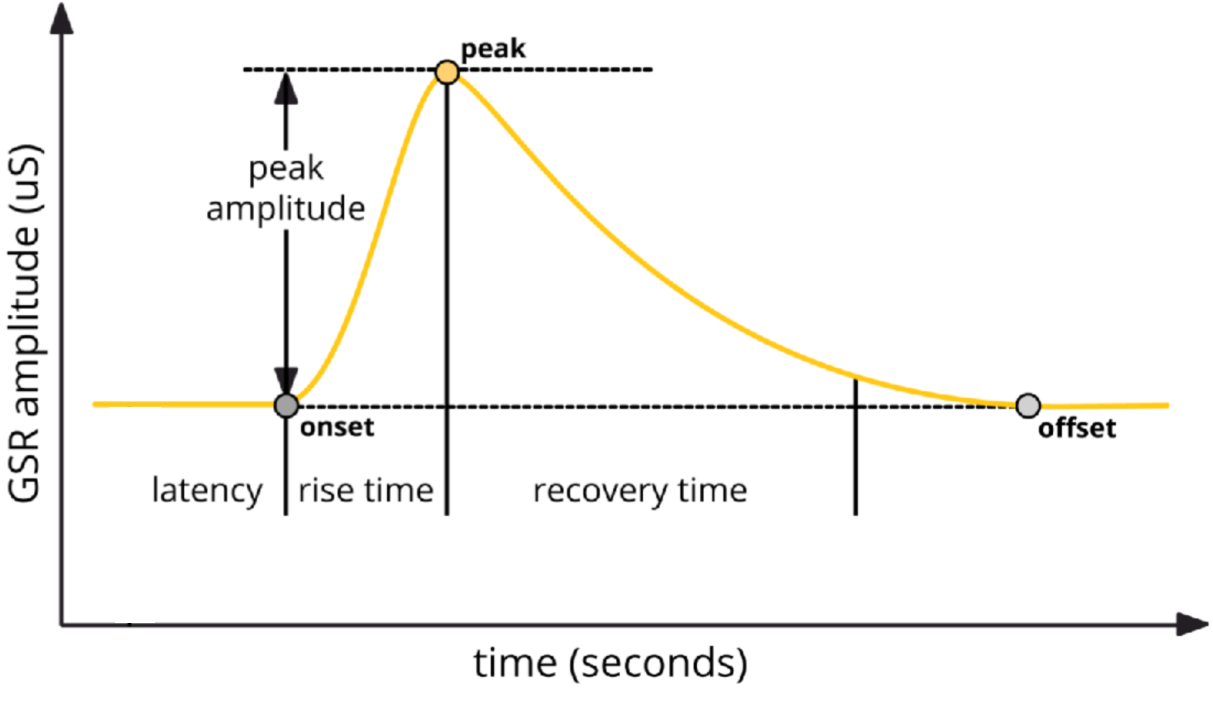
\includegraphics[width=11cm]{Images/peaks.png}}
\caption{ Spitzenzähler: Onset (Startpunkt), Spitze und Offset (Endpunkt). Jedes Paar von Onset/Offset erhöht die Anzahl der Spitzen um eins.} 
\label{fig:peaks} \end{figure} \vspace{0.5cm}


Jedes handgefertigte Merkmal wird auf einem Zeitfenster von Daten für jeden Sensorkanal unabhängig voneinander angewendet. 
Jedes Zeitfenster ist daher 117 Merkmalen zugeordnet (9 Sensorkanäle multipliziert mit 13 Merkmalen). \\





% Unterkapitel 
\subsubsection{Codebook Approach} \label{ca-1}


Die bisherige Methodik mit handgefertigten Merkmalen ist klassisch für den überwachten Lernansatz. 
Es existieren aber auch einige Nachteile. 
Das Hauptproblem besteht darin, dass nicht sichergestellt werden kann, dass die gewählten Merkmale die besten Klassifizierungsergebnisse erzielen. Damit besteht immer die Gefahr, dass möglicherweise andere Merkmalen bessere Ergebnisse liefern würden, diese handgefertigten Merkmale aber die  nicht gefunden wurden. Dieses Risiko besteht insbesondere bei der physiologischen Signalverarbeitung zur Emotionserkennung, wo die Struktur der Daten noch recht unbekannt und allgemein komplex ist. 
Eine weitere Schwierigkeit besteht darin, relevante selbstentwickelte Features ohne Expertenwissen über die Daten zu finden.
Darüber hinaus wurden noch keine gut funktionierenden State-of-the-Art handgefertigten Merkmale identifiziert.
Aus diesen Gründen ist es interessant halbautomatische und unüberwachter Ansätze der Merkmalsextraktion zu verwenden und zu testen. \\


K. Shirahama et al. \cite{kimiaki_codebook_approach_2016} schlugen eine unüberwachte Merkmalsextraktionsmethode namens Codebook Approach (CA) vor, um Merkmale aus 1D-Zeitreihensignalen zu erzeugen.
Der CA hat den Vorteil, dass formbasierte Merkmale gefunden werden können, die für das Problem der Emotionserkennung relevant sind, aber weder offensichtlich noch leicht als Mensch zu interpretieren sind. 
Der CA besteht aus drei Schritten, die in den folgenden Abschnitten erläutert werden: Codebuchkonstruktion (engl. "codebook construction"), Codewortzuordnung (engl. "codeword assignment") und der anschließenden Klassifizierung. \\


\textbf{Codebuchkonstruktion \\}
Ziel dieses Schrittes ist es, Teilsequenzen (sogenannte "Codewörter") zu bestimmen, die für die 1D-Eingangssensorik charakteristisch sind. 
Dies wird erreicht, indem Zeitfenster aus dem ursprünglichen Datensatz für jeden Sensorkanal unabhängig voneinander nach dem im Kapitel \ref{segmenation-1} definierten Segmentierungsansatz extrahiert werden.
Aus jedem so erhaltenen Zeitfenster der Größe $T$ werden kleinere Segmente der Größe $\alpha$ unterteilt.
Ein Clustering-Algorithmus wird dann auf die Menge der Segmente $\alpha$ angewendet, um Clusterzentren zu finden.
Nach der Konvergenz werden die Clusterzentren als Codewörter betrachtet und zum Aufbau einer Sammlung von Codewörtern mit dem Namen ``Codebuch'' verwendet, wie in Abbildung \ref{fig:ca_construction} aus \cite{kimiaki_codebook_approach_2016} dargestellt. 
Die Anzahl der Codewörter (d.h. die Größe des Codebuchs oder die Anzahl der Cluster) ist ein Hyperparameter des Verfahrens. Im Rahmen dieser Arbeit wurde ein k-means Clustering-Algorithmus verwendet, um die Codewörter auf den ELISE-Daten zu erhalten. \\


\begin{figure}[h]\centering{
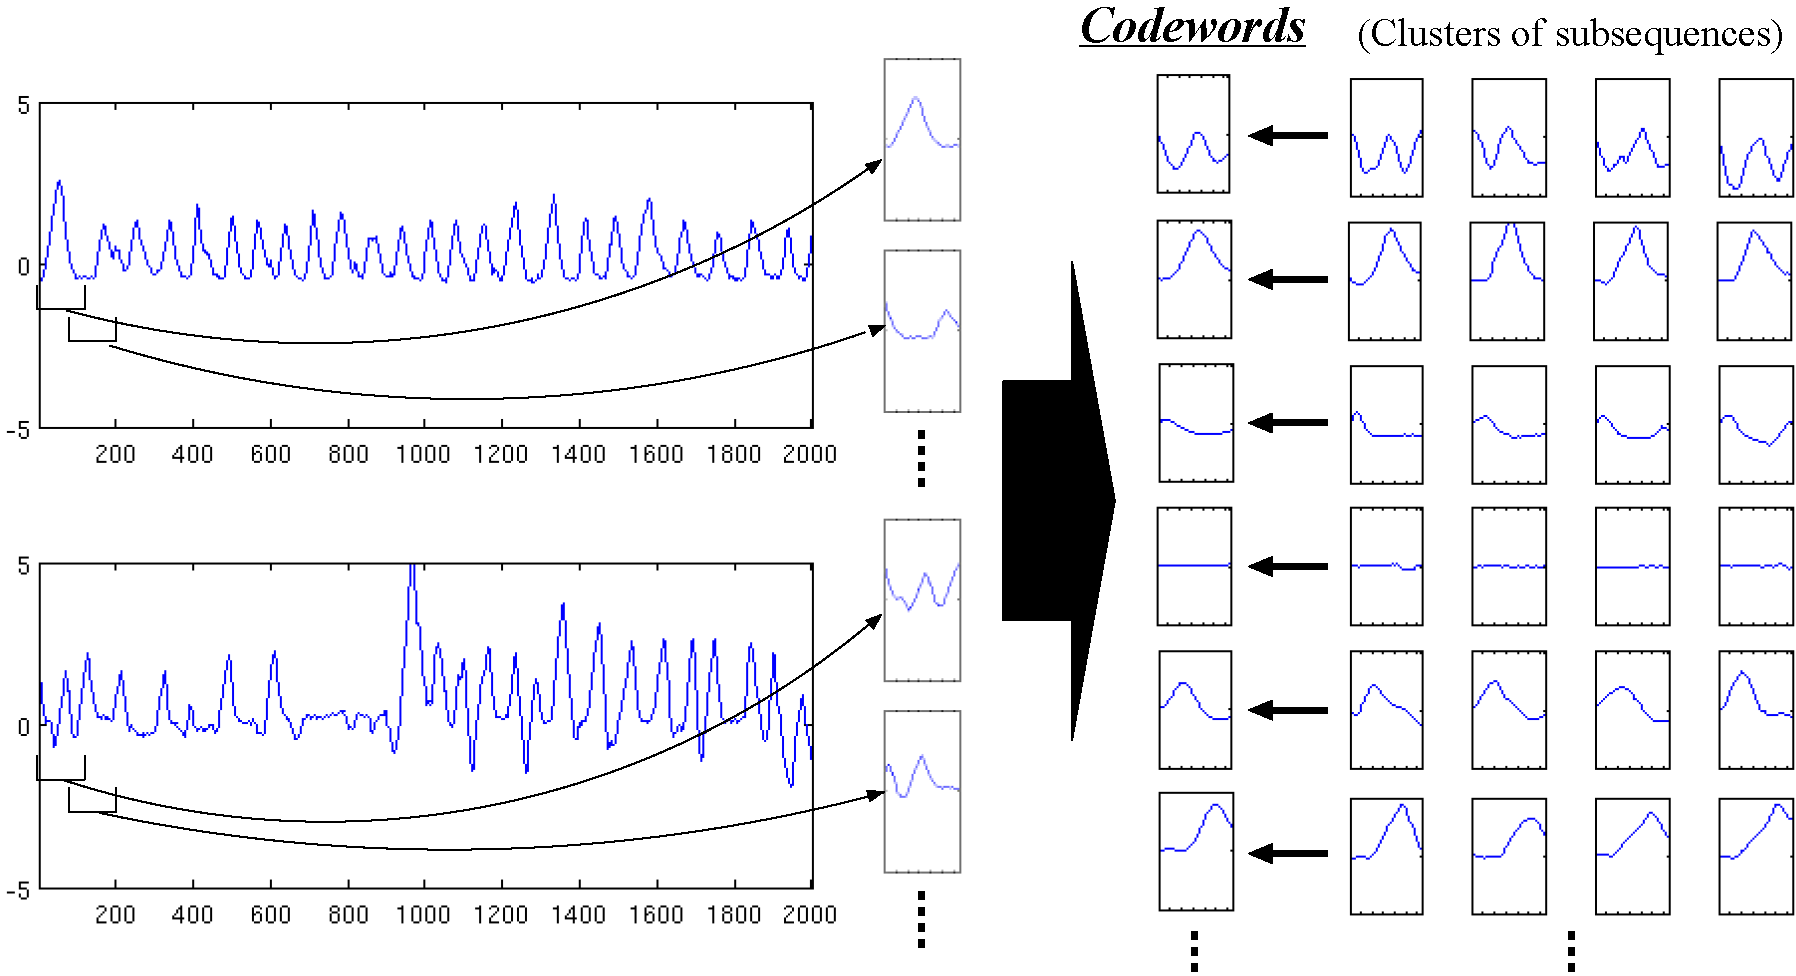
\includegraphics[width=\textwidth]{Images/CA_construction.png}}
\caption{ Codebuchkonstruktion: Zeitfenster von Daten werden zunächst extrahiert. Ein Clustering-Algorithmus wird dann auf das alle Zeitfenster angewendet, um Clusterzentren (und damit Codewörter) zu finden, die zum Aufbau des Codebuchs verwendet werden. }
\label{fig:ca_construction} \end{figure} \vspace{0.5cm}


\textbf{Codewortzuordnung \\}
Nach der Konstruktion der Codewörter wird für jedes Zeitfenster $T$ ein histogrammbasierter Merkmalsvektor erstellt (vgl. Abbildung \ref{fig:ca_assignment}, entnommen aus \cite{kimiaki_codebook_approach_2016}). 
Der zu klassifizierende Datensatz wird zunächst in Zeitfenster der Größe $T$ segmentiert, aus denen Segmente der Größe $\alpha$ nach dem gleichen Verfahren wie beim Aufbau des Codebuchs extrahiert werden. 
Jedes Segment $\alpha$ wird dann mit den Codewörtern verglichen, so dass das "ähnlichste" Codewort gefunden werden kann. 
Ein K-Bin-Histogramm (mit $K$ Anzahl der Codewörter) mit Informationen über die Anzahl der Male enthält, die jedes Codewort als am ähnlichsten zu den Segmenten $\alpha$ im Zeitfenster $T$ betrachtet wurde, wird dann erstellt und als Merkmalsvektor verwendet, um das zu klassifizierende Zeitfenster $T$ darzustellen. 
Das Maß für die Ähnlichkeit von Codewörtern und Datensegmenten $\alpha$ basiert auf der euklidischen Entfernung. \\


\begin{figure}[h]\centering{
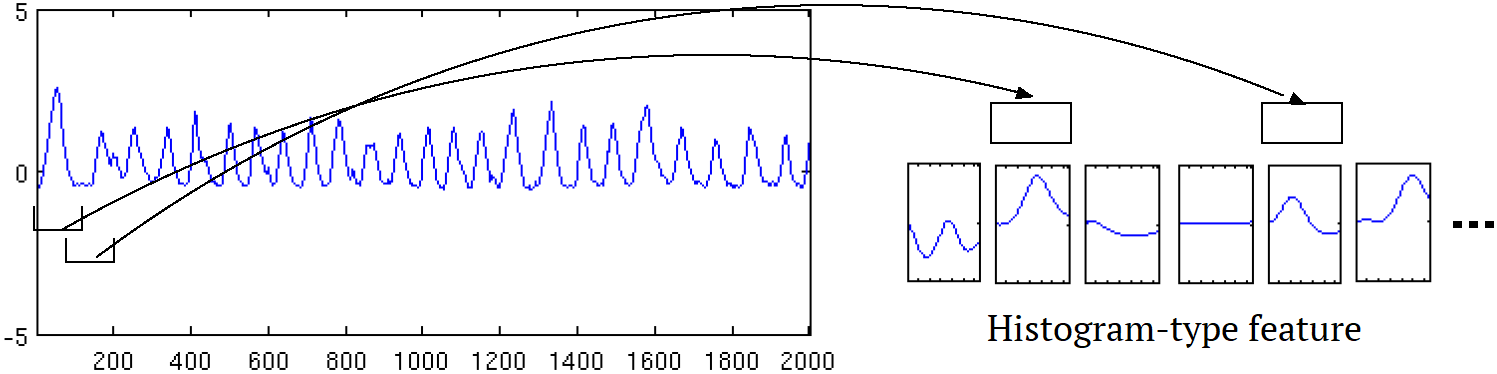
\includegraphics[width=\textwidth]{Images/CA_assignment.png}}
\caption{ Codewortzuweisung: Jedes Datensegment wird mit den Codewörtern verglichen und ein Histogramm mit Informationen darüber, wie oft jedes Codewort als "am ähnlichsten" betrachtet wurde, wird erstellt. }
\label{fig:ca_assignment} \end{figure} \vspace{0.5cm}


Der zuvor beschriebene Ansatz wird als "Hard-Zuordnung" (engl. "hard assignment") bezeichnet, da Datensegmente einem einzigen Codewort zuzuordnen werden.
Ein Nachteil dieser Vorgehensweise ist die mangelnde Flexibilität im Umgang mit potenzieller Unsicherheit bei der Codewortzuweisung, die z.B. auftreten kann, wenn ein Zeitfenster von Daten zwei oder mehr Codewörtern sehr ähnlich ist, da es nur einem zugeordnet werden kann. 
Ein alternativer Ansatz dieses Problem zu umgehen ist die so genannte "Soft-Zuordnung" (engl. "soft assignment"). Hierbei werden auch alle Codewörter des Codebuchs Datensegmenten zuzuordnen, wobei die Ähnlichkeit jeweils als ein Bin im Histogramms dargestellt wird. Sehr ähnlich entspricht hierbei einem hohen Wert und nicht ähnlich einem kleinen Wert (anstatt 0 oder 1 wie in der Variante der Hard-Zuordnung). 
Eine Kerneldichtefunktion (vgl. \cite{gemert_ieee_2009}) wird verwedent, um die Histogramm-Bins zu berechnen. Es wurde die folgende Funktion verwendet:


\begin{equation} 
\Large{ {f(\alpha,c_k,p) = \frac{1}{\gamma}} \frac{g(\alpha,c_k,p)}{\sum_{i=1}^{K} g(\alpha,c_i,p)}}
\end{equation}
\newline
wobei $f(\alpha,c_k,p)$ die Ähnlichkeit des Segments $\alpha$ bezeichnet, das sich auf das Codewort $c_k$ bezieht. $p$ ist ein Glättungsparameter (ein großes $p$ bewirkt eine starke Glättung), $\gamma$ ist die Anzahl der Segmente im Zeitfenster $T$ und: \\
\begin{equation} 
\Large{ { g(\alpha,c_k,p) = \frac{1}{\sqrt{2 \pi p^{ 2 }}}} exp(\frac{d(\alpha,c_k)}{2p^{2}}). }
\label{equ:codeword_assignment_2} \end{equation}
\newline
Um numerischen Unterlauf zu vermeiden, wird die Gleichung (\ref{equ:codeword_assignment_2}) zunächst mit dem Log-Sum-Exp-Trick (vgl. \cite{murphy_2012}) berechnet. \\


\textbf{Fusion mehrerer Sensoren \\}
Oftmals werden mehrere Sensoren verwendet, die gleichzeitig mehrere verschiedene Signale derselben Emotion erzeugen.
Die Fusion dieser Signale ist wichtig, da sie die Genauigkeit der Emotionserkennung verbessern kann.
Es gibt zwei verschiedene Ansätze (vgl. \cite{snoek_2005}): die frühe Fusion (engl. "early fusion") und die späte Fusion (engl. "late fusion"): 

\begin{itemize}
  \item \underline{Frühe Fusion:} In der Dimension $K \times S$ wird nur ein Klassifizierer benötigt, wobei $K$ die Anzahl der Codewörter und $S$ die Anzahl der Sensorkanäle ist. Der Klassifikator wird anhand der Verkettung von Codebuchmerkmalen trainiert und ausgewertet, die auf jedem Sensorkanal unabhängig voneinander berechnet wurden.

  \item \underline{Späte Fusion:} Erfordert mindestens $S$-Klassifikatoren (einen für jeden Sensorkanal). Ein Klassifizierer wird unabhängig für jeden Sensorkanal unter Verwendung der für den betrachteten Sensor erhaltenen Codebuchmerkmale trainiert. Die Vorhersagen der $S$-Klassifikatoren werden dann fusioniert, um die Klassenbezeichnung des zu klassifizierenden Zeitfensters zu schätzen (z.B. mit einem zusätzlichen Klassifizierer).
\end{itemize} \vspace{0.5cm}


In dem ELISE Projekt verwenden wir den späten Fusionsansatz, weil er rechnerisch günstiger ist und von K. Shirahama (vgl. \cite{kimiaki_codebook_approach_2016}) empfohlen wird. \\